\subsubsection{Overfitting to the Data}
\label{sxn:overfitting}
\nred{This section will be re-written completes and merged with parts of 4.1 to make the intoduction to section 4
The objectives are to describe 

\begin{itemize}
\item generally a little about the stat mech approach
\item what is a thermal average, data average
\item  high T, annealed is good enough
\item  the ST model for the error
\item linear perceptron:  error ~ (1-R)
\item phase behavior / meta-stable spin glass states
\end{itemize}

and then to point to the appendix for details as needed
}


In the classic theory of the Statistical Mecahanics of Generalization, \SMOG, if one
trains a simple NN, like an Ising Perceptron, but on very noisy data and/or mislabeled data labels,
or when the model capacity is just too low, the resulting model will be \emph{atypical}
and will effectively overfit to the training data.
This is because the underlying optimization problem is  unrealizable, and,
as the system size grows, the model generalization error $\mathcal{E}^{M}_{g}$ will
remain large and finite, rather than decrease to zero (as expected for a realizable data set).

\begin{figure}[h]
    \centering
    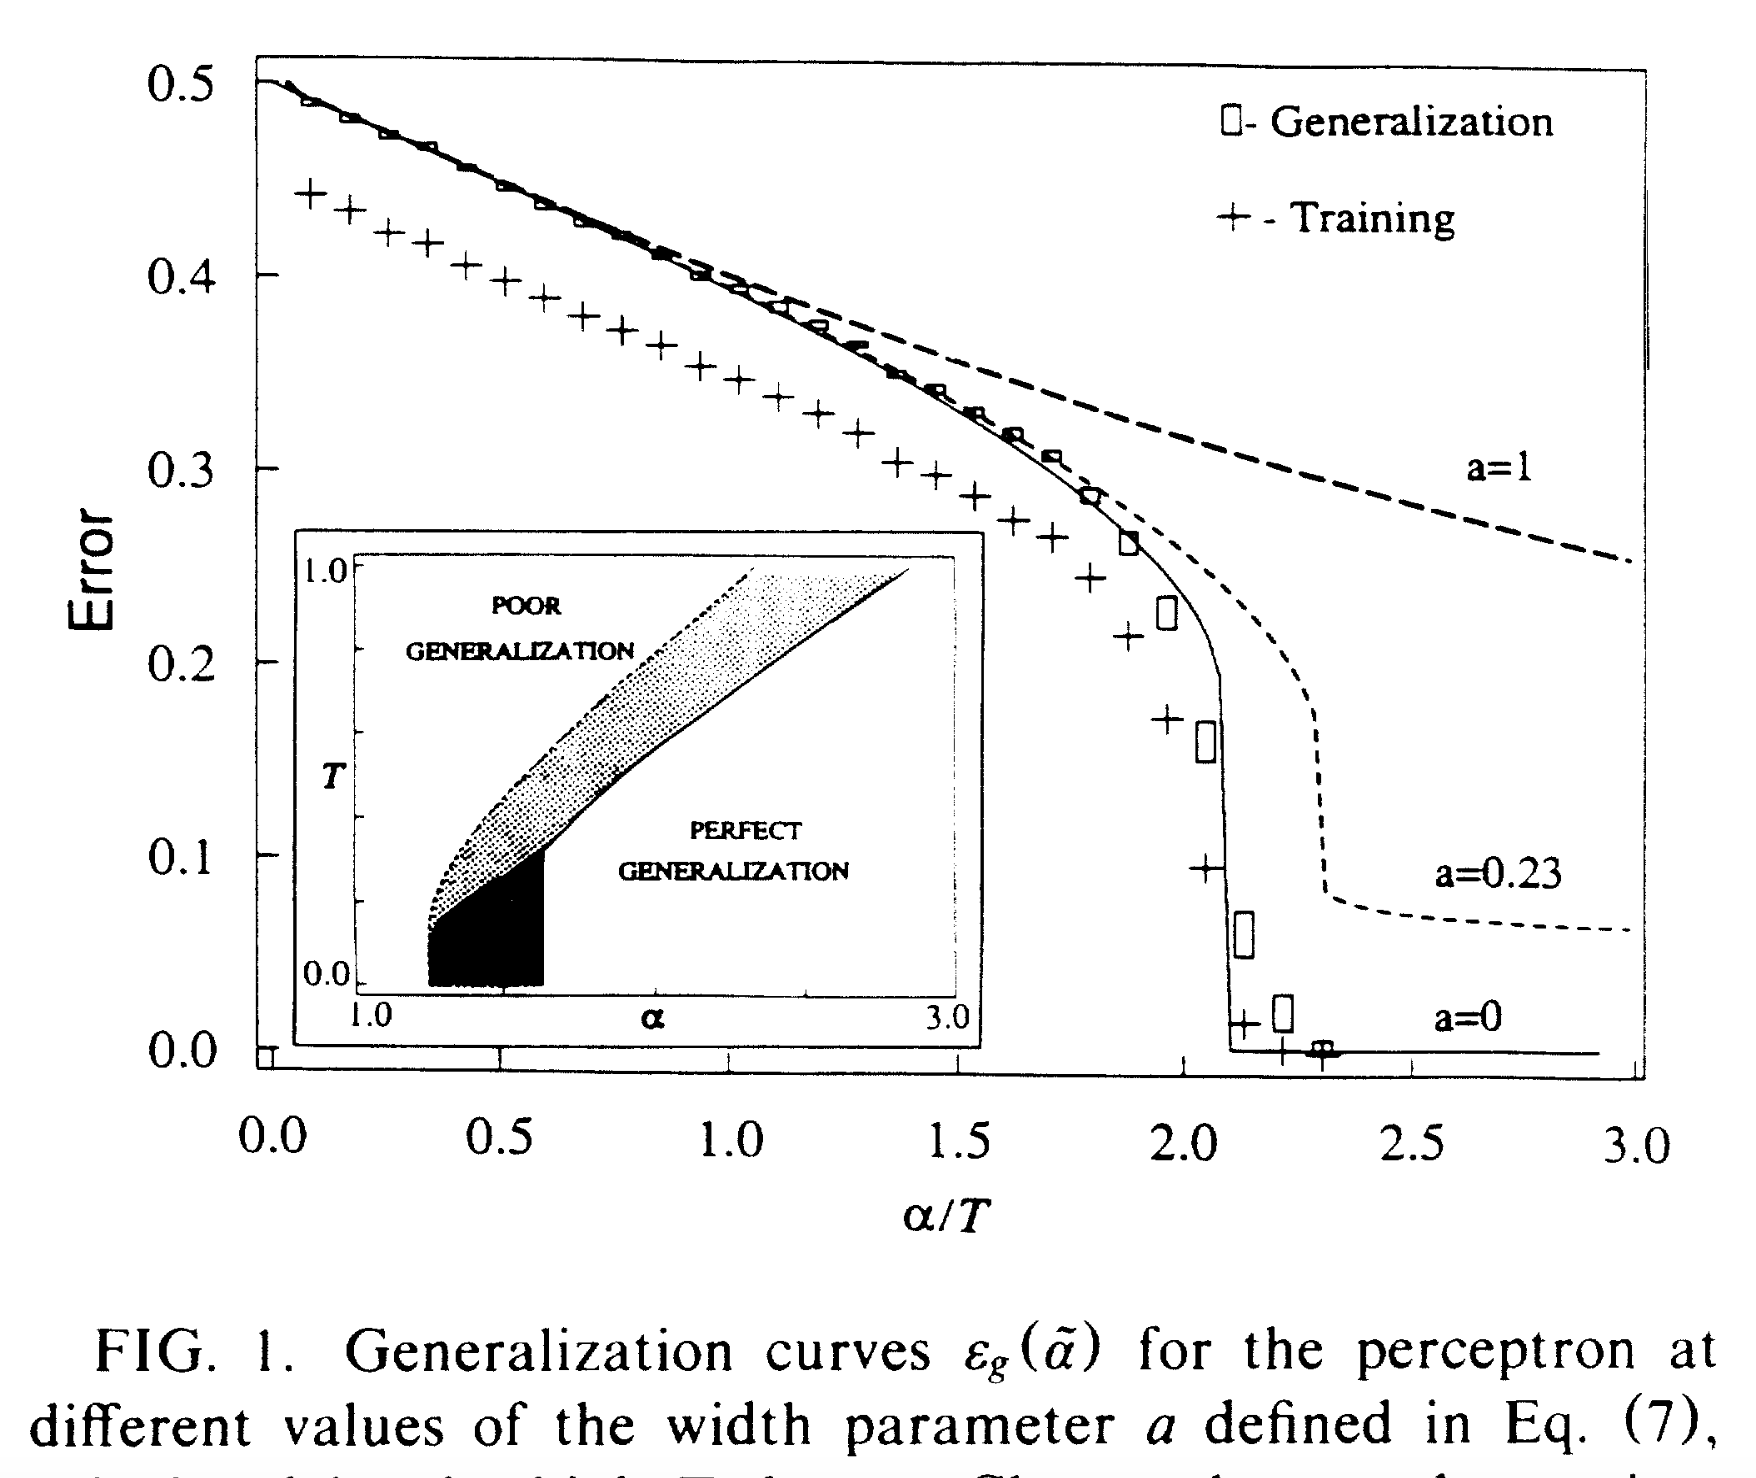
\includegraphics[width=5cm]{./img/SST90-Figure.png}
    \caption{Phase Diagram of the Student Teacher Perceptron Generalization Error. Reproduced from \cite{SST90}}.
   \label{fig:phase_diagram}
\end{figure}


This is depicted in Figure~\ref{fig:phase_diagram}, reproduced from \cite{SST90}.
Here, the x-axis is the load, $\text{load}=N_{D}/N$,
where $N_{D}$ is the number of data examples $N_{D}$, and $N$ is the number of parameters (or weights).
\nred{make 1 or 2 new plots and describe them}

%a discontinuous (i.e first order) phase transition from perfect generalizaiton
%to poor generalzation as the effective number of examples (or load, $\alpha$) decreases.
%(See Figure XXX, reproduced from \cite{ST92}.)

The analytical solution here is a distribution of weights $\mathbf{w}$,
but one which is \emph{atypical}.  That is, these weights can only
only be used to describe the training data (and only very poorly),
and any random draw of $\mathbf{w}$ will more than not fail to
describe any out-of-distribution (OOD) test (hold-out. or validation) example.
And while this can be worked out exactly (i.e in the quenched case with a replica calculstion),
this atypical behavior even occurs in the high-Temperature theory.\cite{SST90}

One can think of the load as proxy for a more general notion of model capacity.
And  when the model capacity is too small, one may expect the model overfits to the training data,
and the layer $\alpha$ to drop below $2$, i.e. $\alpha< 2$.  In this way, one can
directly measure the onset of overfitting in a layer in any trained NN \emph{Semi-Empirically}.

We  simulate such a situation in a small model NN, as shown in Section~\ref{sxn:empirical_fc1}.






